\documentclass[12pt]{extarticle}

\usepackage[T1]{fontenc}
\usepackage{polski}
\usepackage[utf8x]{inputenc}
\usepackage[polish]{babel}
\usepackage{url}
\usepackage{afterpage}

\usepackage[margin=1.1in]{geometry}
\usepackage{color}
\usepackage{graphicx}
\usepackage{float}
\usepackage{indentfirst}
\setlength\parindent{1cm}


\begin{document}
\begin{titlepage}
    \begin{center}
        \textsc{\LARGE{Politechnika Śląska}}\\[0.5cm]
        \textsc{\LARGE{Wydział Automatyki, Elektroniki i~Informatyki}}\\[0.5cm]
        \textsc{\LARGE{Kierunek Informatyka}}\\[5.5cm]
        \LARGE{Wypracowanie z przedmiotu Ekonomia}\\[1cm]
        \LARGE{Autor: Aleksander Grzybowski}\\[1cm]
        \LARGE{Gliwice, kwiecień 2017}\\[1cm]
    \end{center}
\end{titlepage}



\section{Rynek, popyt, podaż}

\subsection{Pojęcie i klasyfikacja rynków}

Rynkiem nazywamy całoksztalt transakcji kupna i sprzedaży oraz warunków, w jakich one przebiegają. Rynek można klasyfikować według różnych kryteriów podziału: według przedmiotu obrotu (dobra i usługi konsumpcyjne), według zasięgu geograficznego (lokalny, międzynarodowy), według sytuacji rynkowej (rynek sprzedawcy/nabywcy), według stopnia jednorodności transakcji (homogeniczny bądź heterogeniczny). Zależnie od stopnia wyrównania cen wyróżnia się rynek doskonały i niedoskonały. Rynek doskonały posiada następujące cechy:

\begin{itemize}
	\item Rozproszenie po stronie popytu i podaży - każdy z podmiotów dysponuje jednakową siłą ekonomiczną i poszczególne podmioty nie mogą wpływać na kształtowanie się cen
	\item Brak barier wejścia na rynek - możliwość łatwego wejścia i wyjścia z rynku
	\item Przejrzystość - zarówno sprzedający i kupujący mają pełne i prawdziwe informacje o towarach i ich cenach
	\item Jednorodność dóbr i usług - dobra o podobnym przeznaczeniu mają podobne cechy fizyczne i są postrzegane przez potencjalnych konsumentów jako jednakowe
\end{itemize}

W rzeczywistości taki rynek występuje bardzo rzadko, zazwyczaj występują mniejsze bądź większe niedoskonałości, które zmieniają obraz rynku. Przeciwieństwem rynku doskonałego jest rynek monopolistyczny - istnieje tylko jedno przedsiębiorstwo, które całkowicie kontroluje produkcję i ceny, mimo to nadal podlega uwarunkowaniom popytu i podaży.

Gospodarka wolnokonkurencyjna charakteryzuje się istnieniem wielu równorzędnych przedsiębiorstw, które w całości mają wpływ na na łączną podaż, ale w izolacji nie kontrolują jej. Pomiędzy poszczególnymi przedsiębiorstwami występuje konkurencja cenowa, a decyzje produkcyjne i handlowe podejmowane są na podstawie bieżącego stanu rynku, przez co w dłuższym okresie czasu przedsiębiorstwa najsilniejsze ugruntowują swoją pozycję na rynku, natomiast słabsze bankrutują i znikają. Zjawisko to można było zaobserwować w ostatnich dziesięcioleciach XIX wieku, kiedy to narastająca walka konkurencyjna doprowadziła do dominacji w większości gałęzi gospodarki kilku przedsiębiorstw najsilniejszych.

Wielki kryzys gospodarczy w latach 1929-1933 zapoczątkował wiele przeobrażeń społeczeństw i gospodarek wielu krajów. Procesy te w istotny sposób zmieniły więzi między podmiotami gospodarczymi. Z obserwacji wynika, że o dojrzałym rynku można mówić, gdy istnieje (1)	 dominacja własności prywatnej i możliwość swobodego transferu praw własności, (2)	możliwość prowadzenia prywatnej działalności gospodarczej, (3) istnienie sprawnie działających instytucji obsługujących rynek (giełdy, banki), (4)  integralność, uniezależnienie się poszczególnych segmentów rynku


\subsection{Funkcjonowanie rynku}

Rynek jest podstawowym regulatorem procesów zachodzących w gospodarce. Podstawową rolą jest dokonywanie wyceny dóbr - cena jest ustalana przez rynek, niejako w sposób naturalny na drodze procesów rynkowych. Rynek stanowi źródło informacji dla przedsiębiorstw - udostępnia wyceny, relacje między cenami, popyt/podaż na dane dobro, informacje o kredytach itp. Jest warunkiem racjonalnego wykorzystania zasobów gospodarczych - dzięki uzyskanym informacjom możliwe jest podejmowanie decyzji opartych na rachunku ekonomicznym i badaniach statystycznych. Pozwala na ustabilizowanie się gospodarki - działania wykonywane przez producentów i konsumentów wprowadzają zaburzenia, które w określonym czasie zanikają. Weryfikuje przydatność produkcji i pozwala na dostosowanie jej do ludzkich potrzeb - efektywny popyt odzwierciedla potrzeby ludzkie, więc badanie popytu pozwala na odpowiednie zaplanowanie produkcji

Rynek rozwiązuje trzy podstawowe problemy każdej gospodarki - co, jak i dla kogo produkować.

\begin{itemize}
	\item  'co' - pozwala na badanie zachowań konsumentów, którzy dokonując zakupu wpływają na popyt
	\item 'jak' - wprowadza mechanizmy konkurencji, dzięki którym możliwe jest utrzymanie jak najniższych kosztów produkcji
    \item 'dla kogo' - pozwala badać dochody konsumentów i odpowiednie grupy docelowe
\end{itemize}

\subsection{Popyt i podaż}

Popyt na dane dobro jest ilością tego dobra, jakie nabywcy są w stanie nabyć po określonej cenie i w określonym czasie. Jest on funkcją wielu zmiennych, głównie ceny, ale także dochodów nabywców, cen dóbr substytucyjnych, gustów nabywców i innych. Zależność między popytem a ceną jest zwykle zależnością odwrotną, to znaczy, wzrost ceny powoduje spadek popytu. Zmiana ceny powoduje dwa efekty: substutycyjny i dochodowy. Efekt substytucyjny polega, w przypadku wzrostu ceny, na skłonieniu nabywcy do rezygnacji z danego dobra i zastąpieniu go dobrem tańszym. Efekt dochodowy powoduje obniżenie dochodu realnego konsumenta - za tę samą cenę możliwe jest nabycie mniejszej ilości dobra. Zależność odwrotna jest typową zależnością występującą na rzeczywistym rynku, jednakże w szczególnych okolicznościach można zaobserwować anomalie, takie jak:

\begin{itemize}
	\item popyt doskonale nieelastyczny - zmiana ceny nie powoduje zmiany popytu, występuje dla produktów, które zaspokajają niezbędne potrzeby i nie mają żadnych substytutów
    \item popyt doskonale elastyczny - zmiana popytu nie powoduje zmiany ceny, występuje przy rynku doskonałym, w którym przy cenie wyznaczonej przez rynek (i tylko tej) przedsiębiorstwo potrafi zrealizować całą swoją produkcję.
    \item popyt paradoksalny - wzrost ceny powoduje wzrost popytu, występuje przy dobrach prestiżowych i w przypadku spekulacji cen
\end{itemize}

Poza ceną, istnieje wiele czynników wpływających na popyt. Jednym z nich są dochody nabywcy. Jeśli wzrastają, popyt generalnie także wzrasta, natomiast w przypadku dóbr podrzędnych może spaść - przykładowo, wzrost dochodów może wiązać się z zmianą preferencji na lepsze jakościowo produkty. Innym czynnikiem są ceny dóbr substytucyjnych i komplementarnych. Wzrost ceny danego dobra substytucyjnego spowoduje wzrost popytu na inne dobro, np. wzrost ceny masła zwiększy popyt na margarynę. Z drugiej strony, spadek popytu na dane dobro spowoduje spadek popytu na dobro komplementarne - przykładowo, wzrost cen samochodów będzie się wiązał ze spadkiem popytu na benzynę.


Podaż danego dobra jest to ilość tego dobra zaoferowana przez producentów do sprzedaży po danej cenie w określonym czasie. Jest ona, podobnie jak popyt, funkcją wielu zmiennych. Podaż i cena zmieniają się w jednym kierunku - wzrost ceny powoduje wzrost podaży. Dzieję się tak, ponieważ wzrost ceny implikuje wzrost opłacalności produkcji, co w rezultacie motywuje producenta do zwiększenia produkcji. Innymi czynnikami wpływającymi na podaż są koszty produkcji (wzrost kosztów produkcji powoduje spadek podaży), rentowność produkcji dóbr substytucyjnych, czy też polityka monetarna bądź sytuacja ekonomiczna państwa. Znaczącą różnicą między popytem i podażą jest czas reakcji na zmiany czynników określających je. Popyt w ogólnym przypadku może zareagować w bardzo krótkim czasie (przykładowo, ludzie nie pójdą do sklepów), podczas gdy podaż reaguje bardzo wolno (zmiana wielkości produkcji może trwać nawet kilka miesięcy).
Wzajemne zmiany popytu i podaży w ramach wahań czynników na nie wpływających są istotą mechanizmu rynkowego, który ostatecznie decyduje o cenie dobra. Każda zmiana czynników wprowadzi do systemu pewne chwilowe zaburzenie, które dzięki działaniom rynku spowoduje powrót do nowego stanu równowagi. Przykładowo, załóżmy, że aktualna cena jest wyższa od ceny równowagi. Spowoduje to nadwyżkę dobra i sytuację korzystną dla nabywcy (popyt mniejszy od podaży). Po jakimś czasie konkurencja między sprzedającymi doprowadzi do spadku ceny, co przywróci stan równowagi między popytem i podażą. Cenę osiągniętą w tym stanie określa się mianem ceny równowagi rynkowej.


\section{Produkcja i koszty w przedsiębiorstwie}

\subsection{Pojęcie i rodzaje przedsiębiorstw}

Przedsiębiorstwo jest podmiotem gospodarczym, który prowadzi działalność produkcyjną, handlową lub usłoguwą w celabh zarobkowych i na własny rachunek. Wielkość przedsiębiorstwa określa się zwykle liczbą zatrudnionych pracowników, wartością produkcji albo majątku trwałego, natomiast kryteria te są zwykle umowne i zmieniają się. W gospodarce rynkowej przewagę stanowią przedsiębiorstwa małe, w przeciwieństwie do gospodarki centralnie planowanej, gdzie prym wiodą przedsiębiorstwa duże. Przedsiębiorstwa rozróżniamy na publiczne (państwowe) i prywatne. Prywatne są zwykle najmniejsze i zwykle opierają się na pracy kierownika i jego rodziny, plus ewentualnie kilku pracowników. Ich zaletą jest niezależność i samodzielność, natomiast poważną wadą jest trudność zgromadzenia większego kapitału, przez co konieczne jest łączenie się przedsiębiorstw i tworzenie spółek.

Spółka jest rodzajem umowy, na mocy której wspólnicy ją zawierający podejmują się prowadzenia wspólnej działalności gospodarczej ku wspólnemu celowi. Wyodrębnia się dwa rodzaje społek: osobowe (jawne, partnerskie, komandytowe, komandytowo-akcyjne) i kapitałowe (spółki z o.o oraz akcyjne).

\begin{itemize}
	\item spółka osobowa - należy do co najmniej dwóch partnerów, którzy ponoszą całe ryzyko związane z prowadzeniem działalności, wnoszą kapitał i odpowiadają za swoje zobowiązania
    \item Spółka jawna - prowadzi przedsięwzięcie zarobkowe we wspólnym imieniu pracowników, w dobrej wierze i w pełnym zaufaniu.
    \item spółka komandytowa - jest odmianą spółki jawnej, w której występują dwa typy wspólników: komplementariusze (odpowiadający całym swoim majątkiem) oraz komandytariusze (odpowiadający tylko do wysokości wniesionych udziałów).
    \item spółka z ograniczoną odpowiedzialnością - składa się ze wspólników, w których wszyscy wspólnicy odpowiadają jedynie do wysokości wniesionego kapitału, który to sumarycznie powinien być nie mniejszy niż 5000 zł.
    \item spółka akcyjna - posiada kapitał w formie akcji, które kupują akcjonariusze, traktując udział w spółce jako pewnego rodzaju lokatę kapitału.
\end{itemize}


Przedsiębiorstwa spółdzielcze są dobrowolnymi zrzeszeniami osób, które prowadzą wspólną działalność w imię swoich członków. W takim przedsiębiorstwie członkowie mogą wnosić udziały także w postaci budynków, maszyn albo ziemi, a zarządzanie opiera się na systemach samorządowych. Podział zysku wykonuje się przy uwzględnieniu wkładu pracy i wielkości wniesionego kapitału.

\subsection{Cele działalności przedsiębiorstwa}

Celem przedsiębiorstwa działającego w klasycznym modelu jest maksymalizacja zysku całkowitego. Aby ten cel zrealizować, określane są rozmiary produkcji i podejmowane są decyzje inwestycyjne. Istnieją też alternatywne teorie, np. w dużych spółkach akcyjnych, w których skomplikowane powiązania między ich częściami regulują inne niż zysk motywacje. 

Zysk całkowity różnicą między przychodami ze sprzedaży a kosztami związanymi z ich uzyskaniem. Utarg całkowity $ U_C $ przedstawia się jako iloczyn ilości sprzedanych produktów $ Q $ i ich ceny $ c $, czyli $ U_c = Qc $ . Wysokość utargu determinowana jest głównie przez popyt oraz pozycję na rynku, natomiast zależności między rozmiarami produkcji a utargiem można rozpatrywać biorąc pod uwagę, w jakim stopniu przedsiębiorstwo ma wpływ na ostateczną cenę. Utarg przeciętny $ U_p $ definiujemy jako średnią cenę sprzedanego dobra, w przypadku stałej ceny jest to po prostu $ c $ .

Jeśli przedsiębiorstwo działa w zakresie rynku doskonałego, nie ma ono wpływu na cenę, którą całkowicie definiuje rynek. Jeśli przedsiębiorstwo zwiększyłoby cenę, to nabywcy zmienili by producenta, natomiast jeśli zmniejszyłoby, nie mogło by sprzedać całej swojej produkcji. W idealnych warunkach utarg przeciętny jest równy utargowi krańcowemu ($ U_p = U_k $). Jednak w typowych warunkach rynek nie jest doskonały, więc przedsiębiorstwa mogą w jakimś stopniu wpływać na poziom cen oraz ilość sprzedanych produktów.

Prowadzenie każdej działalności wiąże się z kosztami. Koszty księgowe to wszystkie faktyczne i udokumentowane wydatki pieniężne, wykonane w trakcie prowadzenia działalności gospodarczej, np. koszty zakupu surowców, płace, opłaty za energię i dzierżawy budynków itp. Nie zawsze jednak pieniądze wydawane są w odpowiedni i optymalny sposób, co wprowadza tzw. koszt alternatywny (koszt utraconych możliwości), czyli równowartość dochodów, które mogłby by być zrealizowane gdyby wykorzystano dany czynnik produkcji w lepszy sposób. Suma kosztów księgowych i kosztów alternatywnych to całkowity koszt ekonomiczny. Z drugiej strony, księgowy jest różnicą między przychodami a faktycznie poniesionymi kosztami księgowymi. Jest on specyficzną formą dochodu, ponieważ nie może być nie może być negocjowany oraz może przyjmować także wartości ujemne, jeśli przedsiębiorstwo przynosi straty.

\subsection{Krótkookresowa i długookresowa teoria produkcji}

Produkcja jest procesem, w którym połączenie różnych czynników produkcji pozwala na uzyskanie określonej ilości produktów. Przedsiębiorca dąży do jak najlepszego wykorzystania czynników produkcji. Zależności między wielkością produkcji a nakładami finansowymi definiowana jest przez tzw. funkcję produkcji $ P_c = f(N_z, N_k, N_p) $ , gdzie kolejne nakłady oznaczają odpowiednio nakłady ziemi, kapitału i pracy. Zwiększenie produkcji wymaga na ogół zwiększenia wybranych nakładów. Ze względu na charakter czynników produkcji, wprowadza się rozróżnienie na czynniki stałe (wolnozmienne, np. powierzchnia produkcyjna) oraz zmienne (np. ilość pracowników).

Krótkookresowa teoria produkcji zakłada, że w analizowanym okresie czasu przynajmniej jeden czynnik produkcji jest stały, innymi słowy, produkcja może wzrastać jedynie dzięki zwiększeniu ilości zmiennych czynników produkcji. Przy zwiększaniu nakładów czynnika zmiennego występuje znane prawo malejących przychodów, mówiące, że ciągłe zwiększanie nakładów będzie dawać coraz mniejsze przyrosty produkcji.

W okresie długim zakłada się, że wszystkie czynniki produkcji są zmienne. W takim czasie możliwe jest podjęcie wielu decyzji, z których najważniejszą jest określenie skali prowadzenia działalności gospodarczej. Przy zwiększaniu nakładów czynników produkcji występuje bezspornie wzrost produkcji, natomiast nie musi to być relacja liniowa. Wyróżniamy 3 możliwości:

\begin{itemize}
	\item stałe efekty skali - rozmiar produkcji rośnie liniowo wraz ze wzrostem nakładów czynników produkcji
	\item rosnące efekty skali - rozmiar produkcji rośnie szybciej niż liniowo wraz ze wzrostem nakładów czynników produkcji
	\item malejące efekty skali - rozmiar produkcji rośnie wolniej niż liniowo wraz ze wzrostem nakładów czynników produkcji
\end{itemize}

\section{Pieniądz. Polityka monetarna}




\section{Bezrobocie}

\subsection{Pojęcie i pomiar bezrobocia}

Bezrobocie oznacza sytuację, w której część osób w wieku produkcyjnym (18-59 lat dla kobiet i 18-64 dla mężczyzn), zdolnych i gotowych do pracy na typowych warunkach występujących aktualnie w gospodarce, pozostaje bez pracy, pomimo jej poszukiwań. W dynamicznej gospodarce rzadko występuje sytuacja, w której wszystkie osoby nalężące do zasobów siły roboczej pracują. Osoby wykonujące pracę najemną (bądź pracujące na własny rachunek) określa się mianem zatrudnionych, natomiast pozostałych - bezrobotnymi. Te dwie grupy w sumie tworzą zasoby siły roboczej. Rozmiar bezrobocia zależy więc od współczynnika aktywności zawodowej, liczby ludności w wieku produkcyjnym i rozmiarów zatrudnienia.

Bezrobocie można wyrażać w wielkościach absolutnych bądź procentowych, najpopularniejszą procentową miarą jest wskaźnik stopy bezrobocia, który określany jest jako stosunek liczby bezrobotnych do zasobów siły roboczej. W Polsce stosuje się dwie metody pomiaru bezrobocia: metoda wykorzystywana w urzędach pracy oraz metoda wykorzystywana w badaniach aktywności ekonomicznej ludności (tzw. BAEL). W metodzie pierwszej bezrobotnymi są

\begin{itemize}
	\item osoby zdolne i gotowe do podjęcia pracy
    \item osoby bez pracy nie uczące się w szkołach (wyjątek - szkoły wieczorowe i zaoczne)
	\item osoby zarejestrowane w urzędzie pracy, jeśli ukończyły 18 lat, nie nabyły prawa do emerytury, nie posiadają gospodarstwa rolnego ani pozarolniczej działalności gospodarczej
\end{itemize}

Bezrobocie traktuje się głównie jako czynnik w danym momencie czasu, jednakże przy takim podejściu ignoruje się procesy zachodzące aktualnie na rynku pracy. Mimo stałego bezrobocia, na rynku pracy dokonują się ustawiczne zmiany, związane z powstawaniem nowych miejsc pracy, zwolnieniami i zatrudnianiami. Aby opisać te zjawiska, należy spojrzeć na bezrobocie od strony strumieniowej, to znaczy na aktualny przepływ osób pomiędzy trzema zasobami: zasobem zatrudnienia, zasobem bezrobocia i zasobem osób nie należących do siły roboczej. W takim przypadku stopę bezrobocia można określić jako stosunek stopy napływu do bezrobocia i stopy odpływu z bezrobocia. Ustalenie, który z tych czynników ma wpływ na ostateczny wynik jest istotny przy wyborze sposobu zaradzenia bezrobociu przez państwo.

\subsection{Ujęcie neoklasyczne}

Twierdzenia stanowiska neoklasycznego zostały sformułowane przez A. Marshalla i A.C. Pigou w wieku XIX. Zgodnie z tym ujęciem, w warunkach gospodarki wolnorynkowej rynek pracy sam dąży do stanu równowagi w miarę upływu czasu. Mechanizm, który zapewnia taką tendencję nazywa się mechanizmem zmian płac realnych. W myśl tego stanowiska, gdyby na rynku pracy powstała nadwyżka podaży przy określonej stawce płac realnych, to konkurencja między pracownikami doprowadziłaby do zmniejszenia się płac, w rezultacie czego podaż zmniejszyłaby się i nierównowaga zostałaby zlikwidowana.

Teoria neoklasyczna tłumaczy istnienie bezrobocia ograniczeniami w swobodnym działaniu mechanizmu rynkowego, powodowanymi przede wszystkim przez związki zawodowe, które usztywniają płace i opierają się ich zmniejszaniu. Gdyby płace realne ustaliłyby się powyżej niż płace równowagi, a jednocześnie związki zawodowe blokowałyby tę zmianę, powstanie bezrobocie związane z nadwyżką podaży nad popytem. Takie bezrobocie określa się mianem bezrobocia dobrowolnego, ponieważ jest ono dobrowolnie tworzone przez pracowników, którzy nie akceptują działania mechanizmu rynkowego. W takim rozumieniu, aktywna ingerencja państwa w procesy zachodzące na rynku pracy nie jest wymagana do zwalczania bezrobocia, zamiast tego potrzebna jest likwidacja ograniczeń działania mechanizmu rynkowego (zmniejszenie roli związków zawodowych, zwiększenie elastyczności płac).

Ujęcie neoklasyczne budzi wiele wątpliwości, głównym problemem jest zbyt gorliwa wiara w działanie mechanizmu rynkowego, w szczególności mechanizmu płacowego. Innym zarzutem jest obarczanie winą związków zawodowych.









\section{Inflacja}

\subsection{Definicja}

Literatura ekonomiczna definiuje inflację na różne sposoby. Jest to spowodowane chęcią jednoczesnego wytłumaczenia przyczyn tego zjawiska, które jest dość kontrowersyjne ze względu na różne poglądy. Ogólnie przyjmuje się, że inflacja jest wzrostem ogólnego poziomu cen. Warto zauważyć, że inflacja jest dłuższym procesem, tak więc występuje wtedy, gdy wzrost cen ma charakter względnie trwały. Jeśli ceny zmieniają się gwałtownie (np. na skutek wprowadzenia nowego prawa albo zniesienia dotacji na produkcje danego dobra), to takiego wzrostu nie traktuje się jako inflację. Odróżnienie tych dwóch przypadków zwykle nie jest łatwe od razu, potrzebny jest upływ czasu do wyciągnięcia sensownych wniosków.

Zmiany poziomu cen obliczane są w polsce przez Główny Urząd Statystyczny (GUS). W tym celu konstruuje się tzw. wskaźnik cen, który jest pewnego rodzaju miarą zmian wydatków związanych z zakupem pewnego stałego zestawu dóbr (tzw. koszyka) w jakimś czasie. Koszyk dóbr pozostaje zawsze taki sam, tak więc zmiana ceny koszyka wynika wyłącznie ze zmiany cen dóbr zawartych w koszyku. Jeśli istnieje potrzeba zbadania inflacji z punktu widzenia konsumentów, w koszyku należy uwzględnić zwykłe dobra i usługi konsumpcyjne, takie jak żywność, odzież, media czy transport, natomiast z punktu widzenia gospodarki analizuje się wszystkie dobra i usługi wchodzące w skład PKB kraju. Przy wyznaczaniu wskaźnika cen wykorzystywana jest średnia ważona, której wagi odpowiadają ekonomicznemu znaczeniu danego dobra. Wynikiem takich rozważań jest wskaźnik stopy inflacji, który definiowany jest dwojako: 

\begin{enumerate}
	\item porównanie ogólnego poziomu cen z roku poprzedniego z poziomem cen z roku aktualnego, po uśrednieniu wszystkich wskaźników z 12 miesięcy
    \item porównanie poziomu cen z miesiąca grudnia roku poprzedniego i aktualnego
\end{enumerate}

Procesy inflacyjne mierzone wskaźnikami cen mogą mieć różny stopień nasilenia. Inflacja pełzająca występuje, gdy wskaźnik cen jest mniejszy niż 5\% rocznie. Dla przedziału 5-10\% występuje inflacja umiarkowana, dla 10-150\% inflacja galopująca, natomiast powyżej mówi się już o hiperinflacji. Niestety, wszystkie wskaźniki określające inflację mają pewne wady. Głównym problemem jest deaktualizacja wag stosowanych przy ich obliczaniu, innym jest brak wychwytywania zmian jakości dóbr i usług znajdujących się w koszyku.

\subsection{Skutki inflacji}

Poglądy na temat skutków inflacji nie są całkowicie jednolite. Wśród opinii negatywnych można wyróżnić też pozytywne. Częstym poglądem występującycm w literaturze jest pogląd mówiący, że powolne procesy inflacyjne mają korzystny wpływ na przebieg procesów gospodarczych. Według tej opinii, powolne procesy inflacyjne wspomagają dynamikę rozwoju gospodarczego, ponieważ obniżają realne stopy procentowe i stawki płac realnych, co wpływa na nastroje przedsiębiorców i poprawę rentowności produkcji. Co więcej, procesy inflacyjne ułatwiają zmiany relacji cenowych w warunkach sztywnych cen od dołu. Relatywny wzrost cen pewnych dóbr jest procesem naturalnym, natomiast ich spadek realizuje się dzięki stabilizacji cen, w związku z tym inflacja przyspiesza ustalanie się właściwych relacji cen.

Wśród negatywnych skutków inflacji wymienić można zniekształcenie informacji rynkowych (brak wiarygodnych informacji o cenach), spadek popytu na pieniądz i zwiększenie niepewności w zakresie przewidywań zmian cen. Jeśli ceny rosną, rachunek ekonomiczny znacznie się komplikuje i podmioty gospodarcze mają problem z ustaleniem dobrej ceny.

\begin{figure}[H]
\centering
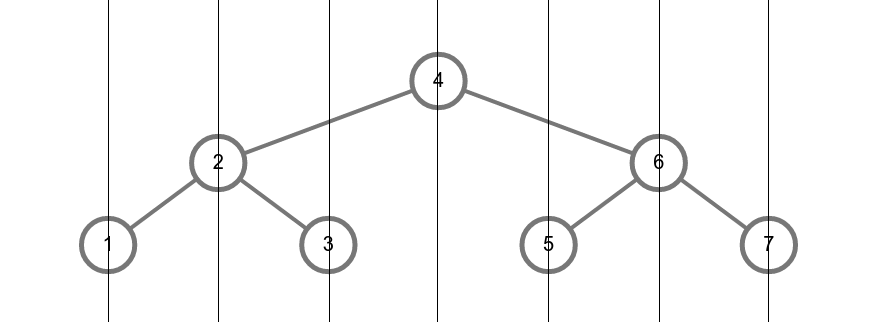
\includegraphics[width=15cm]{sample}
\caption{Jakiś obrazek}
\end{figure}


\begin{enumerate}
	\item Jakaś
	\item Lista
	\item Jakaś
	\item Lista
	\item Jakaś
	\item Lista
\end{enumerate}

\clearpage\mbox{}\clearpage
\end{document}
